\section{The SEA Technique}
\label{SEC:approach}

\begin{figure}[t]
  \center{}
  \fbox{\includegraphics[scale=.37]{images/approach}}
  \caption{Using SEA allows developers to capture features that make an
    environment problematic and use them to prevent future applications
    from falling victim to the bugs of the past.}
  \label{figure:approach}
\end{figure}

The Simulating Environmental Anomalies (SEA) technique
offers a methodical way to
capture, store, and utilize the insights gleaned from
previous failures in a given environment.
In this section, we offer a high-level look at how
SEA works, as illustrated in Figure~\ref{figure:approach}.
This is followed by a more in-depth look at its primary operations,
and the details of our concrete implementation, CrashSimulator.

\subsection{SEA in a Half-shell}
\label{SEC:SEAHalfshell}
In brief,
here is how the technique works.
An application, $A$, is run
in a particular environment and fails.
In debugging the failure,
we identify and ``trap'' the particular environmental feature
(sec.~\ref{SUBSUB:IdentifyingAndEncoding}),
that caused the failure,  which we call $X$.
We verify that when $X$ is present,
the results of interactions with the
environment are different,
sometimes in a barely perceptible manner,
and other times in a radically contrary manner.
We call this difference $\Delta X$.
$\Delta X$ can be extracted, preserved,
and later used in testing other applications
thanks to a pair of components referred to as a mutator and a checker.
The mutator, $mutX()$,
is able to apply $\Delta X$
to the appropriate places in an application's interactions
in order to simulate the presence of $X$.
The checker, $checkX()$ describes how an
application should respond once $X$ has been encountered.
To test if another application, $B$, also has a problem with $X$,
$mutX(B)$ is used to apply $\Delta X$ to its interactions
(sec.~\ref{SUBSUB:MutatingCommunications}).
$checkX(B)$ is then used to determine whether
$B$ has responded correctly to $X$(sec.~\ref{SUBSUB:CheckingResponse}).
If the checker accepts $B$'s behavior
after $X$ is simulated,
we report it has been handled correctly.
If the checker doesn't accept, we report that it has not responded correctly.
Once created,
these pieces act as the persistent medium in which the details of
a given anomaly are stored.

Representing an anomaly in terms of mutators and checkers
allows it to be easily reused to test other applications
without per application effort.
While an application's test suite is typically
tightly coupled to the programming language
and frameworks with which it was written,
SEA's approach is agnostic to these features.
This means anomalies that were useful in testing one application
can be programmatically applied toward testing another.
In this way, SEA is able to augment application-specific test suites
by both decreasing the number of tests
that must be manually constructed
to cover environmental concerns
and by offering the possibility of catching
failures that had not been considered.
These anomalies can be accumulated from many applications
resulting in the ability to test new applications
against an ever increasing
set of problematic conditions.

\subsection{Primary Operations}
\label{SEC:PrimaryOperations}

To take a closer look at how SEA functions,
we divide the technique
into its three primary operations.
These are:
identifying and trapping anomalies,
mutating system call results,
and checking application responses.

\subsubsection{Identifying and Encoding Anomalies}
\label{SUBSUB:IdentifyingAndEncoding}
Building a corpus of anomalies
is an ongoing process that improves the technique's
effectiveness by extending the set of problematic features it can simulate.
Anomalies can be sourced
in a number of ways,
such as
examining the failures of other applications
in a target deployment environment,
or by using other tools that can identify
potentially problematic behavior in other domains~\cite{Zhuang_NSDI_2014,
rasley2015detecting}.
Another option is taking this information from
public bug trackers, which is ideal
if you wish to determine
whether or not an application
is vulnerable to a widely publicized bug.

The chosen anomalies are examined
to determine how they change the results
of system calls an application makes as
compared to a normal execution.
Once teased out,
these differences delineate
a set of modifications
that must be made to an execution
in order to simulate the chosen anomaly or anomalies.
These details are used to
construct both a mutator and a checker.
The mutator encodes
a description of when in execution an anomaly can be simulated,
as well as details of how to conduct that simulation.
The checker
(or set of checkers)
stores a characterization of
how the application should respond.
Describing anomalies in this fashion
allows them to be recorded systematically and cataloged for future use.

As an example, consider
an anomalous environment
where access to a required file is denied because of
the environment's file security configuration.
With this anomaly,
attempts to access the file,
such as
the {\tt read()} system call,
will fail with an error stating that access to the file is denied.
The mutator derived from this issue would be constructed to
identify similar accesses as opportunities
to insert the anomaly
by making these
accesses return ``access denied''.
As described in \ref{SUBSUB:CheckingResponse},
an associated checker would be built to
examine the application's behavior after a simulation and assess its
correctness.
Preserving the details of anomalies like this in the form of
mutators and checkers
allow them to be
easily used
to test responses of future applications.

Constructing new checkers and mutators is a creative process not unlike
writing a unit test.  The writer must understand both the cause of
misbehavior in a deployment environment and how it is visible in the
results of the system calls an application makes.  Once they have this
understanding, the actual construction boils down to building state
machines that recognize the required patterns of system calls.  As a
result, effort required by this process depends on the complexity of the
anomaly being simulated and the proficiency of the writer with the above
concepts.

\subsubsection{Mutating System Call Results}
\label{SUBSUB:MutatingCommunications}
Simulating an environmental anomaly requires specific interventions at the
correct moments during an execution.
These situations are identified
with the help of the chosen anomaly's
mutator.
For our work,
this means providing
the mutator
with the system calls
an application makes
so it can identify sequences
indicative of such opportunities.
At the appropriate time,
the application's system calls
are intercepted
and the mutator's anomaly description is used to
make the modifications necessary
to simulate the anomaly.
In the simplest case,
simulating an anomaly only requires
the modification of a single value
(e.g. {\tt read()} returning -1 rather than the number of bytes read).
We even found use for a ``null mutator''
that performs no mutation, but gives other tools an opportunity to examine an execution.
In more complex cases,
large numbers of diverse system calls
will need to be interdicted and altered
in order to provide a correct simulation.
The above file access scenario, for example,
requires the modification of a single system call.
Simulating something more complex,
like an unreliable system clock,
requires that all efforts
to access the clock
be modified to reflect the chosen aberration.

\subsubsection{Checking an Application's Response}
\label{SUBSUB:CheckingResponse}
SEA relies on checkers
to provide a flexible approach to assess the way an application
behaves after it has encountered an anomaly.
A checker models
the behavior an application should undertake
in response to a simulated anomaly.
It looks for this behavior by examining an application's system calls
before, during, and after simulation.
The checker then reports whether the application has handled
the anomaly correctly
based on whether it observed the behavior for which it was built to look.

As an example, consider the ``default checker'' from CrashSimulator.
It draws a conclusion based on
whether or not the application
has made an effort to respond
to the anomaly.
This determination is made based
on the assumption
that such a response will yield
different program paths, and therefore different system calls.
If the application
does not alter its behavior, it has not
correctly handled the anomaly.
Alternatively,
if the application does deviate,
it is likely
an action has occurred to handle the simulated condition.
This simple yes or no approach
is often sufficient
to classify application behavior.

We explore this, and other checkers in our
Evaluation section (Section VI)~\ref{SEC:evaluation}.
Section~\ref{sec-move-bugs} demonstrates how to find bugs using the null
mutator, while Section~\ref{sec-file-type-bugs}
illustrates how a more complex
mutator can simulate specific scenarios to see if unexpected problems
emerge.

\subsection{Building Checkers and Mutators: A Real-World Example}
\label{SUBSEC:Example}

\begin{figure*}[t]
  \center{}
  \fbox{\includegraphics[scale=.17]{images/curlflow}}
  \caption{Curl examines the {\tt stdout} and {\tt stderr} file descriptors
  and alters the format of its output based on what it finds.  It does this
  to improve usability by outputting a progress bar while being careful to
  avoid corrupting the data it is downloading when both {\tt stdout} and
  {\tt stderr} refer to the same file.}
  \label{figure:curlflow}
\end{figure*}

\begin{figure}[t]
  \center{}
  \fbox{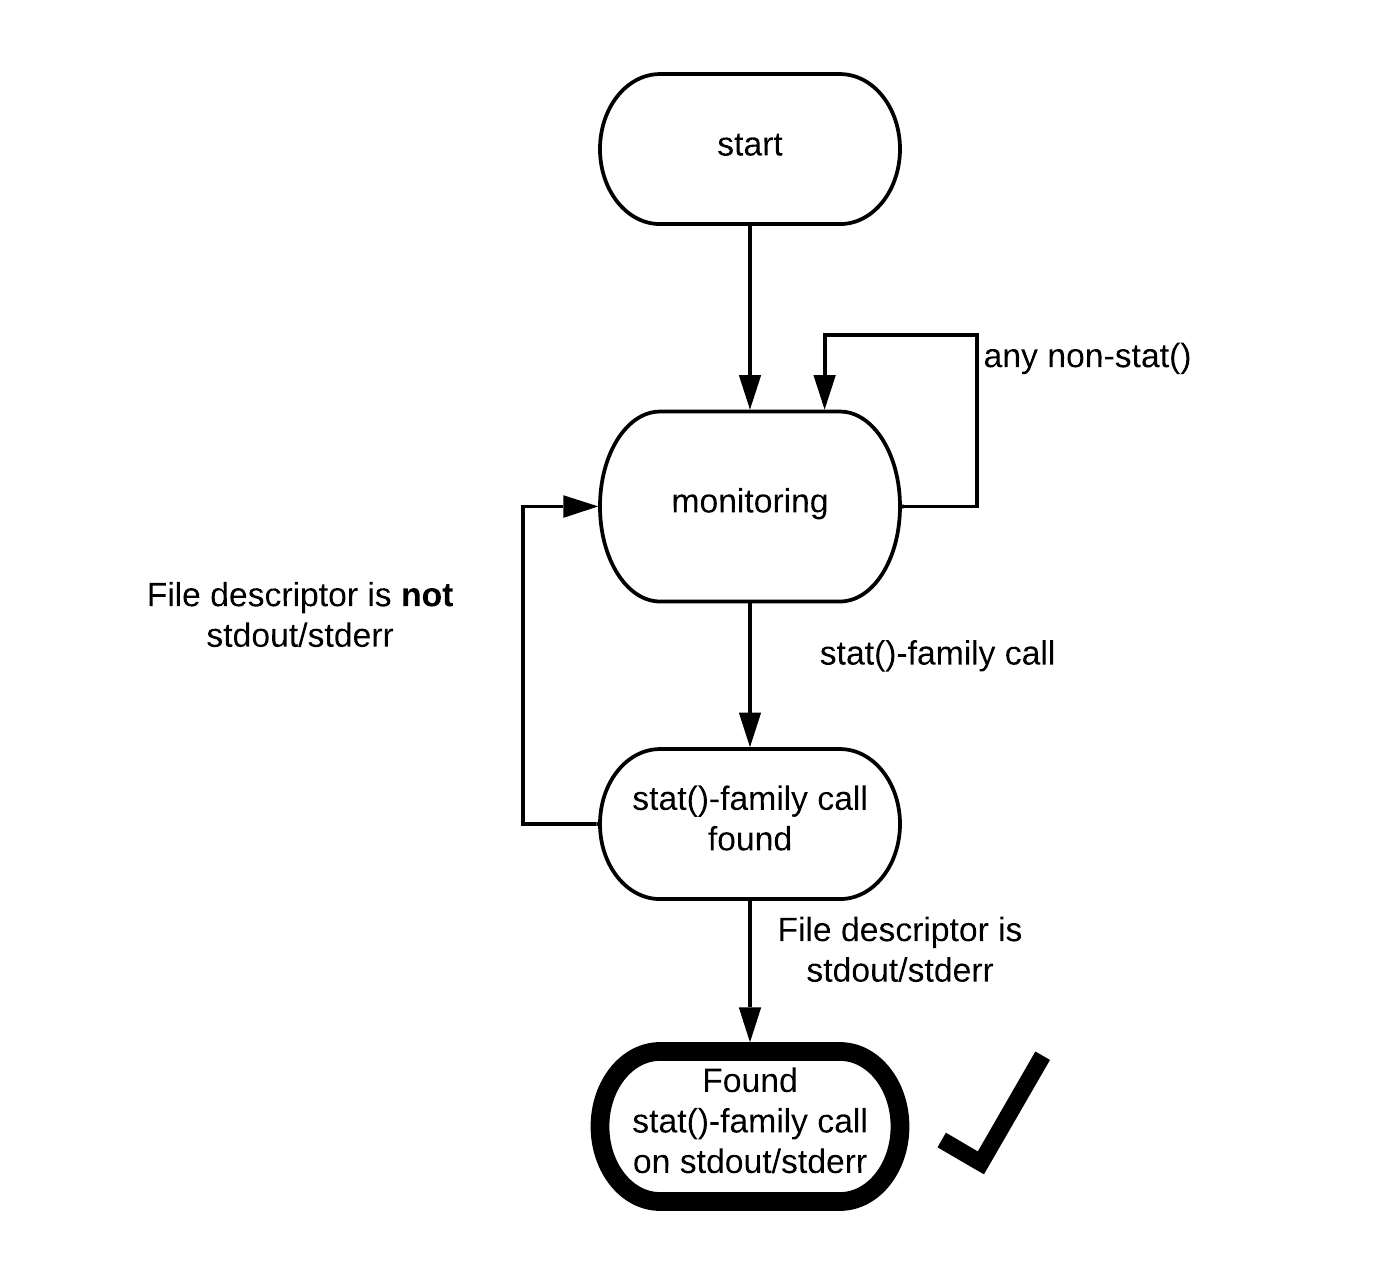
\includegraphics[scale=.6]{images/statidentify}}
  \caption{A mutator simulating the combinations of character devices and
  regular files curl handles must identify a call from the {\tt stat} family
  operating on the {\tt stderr} or {\tt stdout} file descriptor.  It
  can then modify the returned structure to simulate a given combination.}
  \label{figure:statidentify}
\end{figure}

As a real-world example
of building checkers and mutators
consider the measures {\tt curl} takes
to ensure it properly outputs the data it retrieves from a URL.
By default,
{\tt curl} outputs the contents of the requested URL to the terminal.
In cases where {\tt stdout}
refers to a file, {\tt curl} instead outputs a progress bar to the terminal by
writing to {\tt stderr}.  In a third case where both {\tt stdout} and {\tt
stderr} are redirected to files, {\tt curl} omits this progress bar entirely.
This is to prevent interference
interfere with the data being retrieved from the URL if {\tt curl}'s
user specifies a configuration in which both {\tt stdout} and {\tt stderr} are
redirected to the file.

{\tt Curl} determines the configuration of {\tt stdout} and {\tt stderr}
by using a system call from the
{\tt stat} family.  Specifically, calls from this family return a structure that
contains, among other information, a bitmap that denotes the Linux file type of
the file being examined.  Evaluating this bitmap allows an application to
determine whether a file descriptor points to a data file
(a regular file) or the terminal (a character device).
Well-behaved applications should make these checks and alter their output accordingly.

Figure~\ref{figure:curlflow} illustrates the combinations of regular files and character devices
that {\tt curl} looks out for.  SEA allows for the construction of a mutator and
a checker that can test other applications against the same set of
combinations.  Such a mutator would identify {\tt stat}-family system calls
performed upon the {\tt stdout} and {\tt stderr} file descriptors and alter
their results to simulate the desired combination.
See Figure~\ref{figure:statidentify}
for a diagram of a potential underlying automaton for this mutator.
Some indication of the
correctness of an application's response to the simulation could be gained by a
checker that simply looks for the application to change its behavior in
unexpected cases (i.e. the default checker).


\subsection{CrashSimulator: A Concrete SEA Implementation}
\label{SUBSEC:ApproachCrashSim}

In order to correctly implement SEA, CrashSimulator
must provide a framework
by which the checkers and mutators
constructed by its users can be used to
test an application using the anomalies they represent.
Building this capability
required making a few key design decisions. The first, as mentioned in
Section 2, was choosing to operate at the system call level, rather than
manipulating calls to library functions, memory accesses, or other points
where we could influence an application's interactions.
This allowed CrashSimulator
to test applications written in any
language that can execute Linux system
calls -- an important advantage as our
goal is a tool that can test many
applications without per application
effort.
Working with system calls is also a good fit
for simulating the file system,
network, and operating system anomalies in which we were interested.
An application normally queries these entities using system calls
so we simply had to return modified responses in order to simulate an
anomaly.
Finally, robust tooling in the Linux kernel made the
interception and modification of system call results and side effects a
fairly simple process,  and the well-defined semantics of Linux
system calls streamlined implementation.


In order to take advantage of our ability to simulate anomalies using
system calls, we needed to ensure that an application would reliably make
the same set of
system calls, and reach the same simulation opportunities,
with every execution.
To this end,
we employed a modified
{\tt rr} debugger~\cite{rrwebsite} to record and replay applications. Our
first modification permitted a {\tt strace}-style system call recording
to be output alongside {\tt rr's} normal recording format,
creating a complete log of an application’s system call activity.
We chose to make this
modification because, while {\tt rr}'s recording contains the system call
information we need, it is stored in an opaque format that changes
frequently between versions.  Storing a copy of this information as a {\tt
strace} recording bypasses this shortcoming and offers the advantage of
being human readable.

Our second modification parallelized our testing
by allowing {\tt rr} to generate copies of a running application when
it reaches our target simulation opportunities.
We refer to this new technique as {\it process set cloning}
and illustrate it
in Figure~\ref{figure:architecture}.
The {\tt rr}
debugger manages, and can copy, the full set of processes underlying an
application so that users can test debugging hypotheses without damaging
the original.  We extended this capability by liberating process
set copies from {\tt rr}.  This means that given application $Y$ consisting
of processes $a$, $b$, and $c$ (written as $Y(a, b, c)$), we can generate
cloned sets $Y_1(a_1, b_1, c_1)$, $Y_2(a_2, b_2, c_2)$ ... $Y_n(a_n, b_b,
c_n)$.  $Y_1$, $Y_2$ ... $Y_n$ can then be used to test different
scenarios.  These clones can be run in parallel because they do not
actually execute system calls or modify the operating system state.
Instead, they are simulated as described below.
Additionally,
they allow the original $Y$ to continue its execution unhindered.

Once generated, the cloned process sets are used
for testing by the CrashSimulator process supervisor.
This supervisor is responsible for attaching to a process set
via {\tt ptrace} and
servicing any system calls it makes.
The data required to service these calls
comes from the  {\tt strace} log
generated by {\tt rr}.
Just before it takes over service of system calls,
the process supervisor invokes the intended anomaly's mutator
on the log in order to alter it to include the responses
necessary to simulate an anomaly.
Once these alterations are in place,
the supervisor is able to impose an anomaly
on the application by returning the now-modified responses from the log.

During this process,
a corresponding checker
monitors the application's behavior,
allowing it to report on the correctness of the response.
For example, testing could proceed in the following way.
At a given simulation opportunity, when executing application $Y$,
cloned sets $Y_1$ and $Y_2$ are generated and
used to test two scenarios where a file access could fail:
\begin{enumerate}
    \item{For $Y_1$, access to the file is denied due to a permissions issue}
    \item{For $Y_2$, access fails because of an I/O error}
\end{enumerate}
The simulations for both $Y_1$ and $Y_2$ are handled asynchronously and
the results are recorded.
This approach allows many tests to be run independently of one another,
which lends a
high degree of speed and
parallelism to the testing process.
At the same time, the original $Y$ execution continues unhindered to the
next simulation opportunity where this process repeats.
Keeping the original execution intact,
as opposed to destroying it by introducing an error state,
avoids the penalty
of having to restart a new execution for each test.

\begin{figure}[t]
  \center{}
  \fbox{\includegraphics[scale=.37]{images/architecture}}
  \caption{Diagram illustrating CrashSimulator's architecture.  During the
    course of a single rr execution, clone process sets are generated at
    specific rr events.  A CrashSimulator process supervisor attaches to
    these process sets and uses a strace-style system call listing to feed
    subsequent system call activity and inject unusual environmental
    conditions.}
  \label{figure:architecture}
\end{figure}

The prototype was built on rr version 5.2.0 running on a 32-bit Linux kernel
distributed with Ubuntu 16.04 LTS.  The modifications to rr described above
were carried out in C++, and the CrashSimulator
supervisor was implemented in 6260 lines of Python 2.7 code with a 2125
line C extension that allows it to interact with processes using the Ptrace
API.
This version of CrashSimulator is available at:
https://github.com/pkmoore/rrapper.
